
\documentclass[11pt]{article}
\usepackage{amsmath, amssymb, graphicx}
\title{Incremental Zero-Free Symmetry in Weighted NB/BD Framework -- v13.6}
\author{Serabi (Heuristic Record)}
\date{\today}

\begin{document}
\maketitle

\begin{abstract}
We present v13.6, the incremental extension of our heuristic path toward the Riemann Hypothesis (RH).
With $\varepsilon = 0.11$, the zero-free region boosts $\eta$ by 60\% to $\eta \approx 0.56$, yielding a
positivity flip in $\theta$ up to $0.380$. This enhancement stabilizes decay measures and suggests improved
asymptotic convergence through Möbius oscillation and functional equation symmetry.
\end{abstract}

\section{Introduction}
Following v13.5, we extend to $N=5\cdot 10^7$ with incremental zero-free enhancement.
Our calibration uses $c_0 \approx 0.7$ from Pólya--Vinogradov bounds and an initial $\eta \approx 0.35$,
boosted by 60\% to $\eta \approx 0.56$.

\section{Numerical Scaling}
Base regression (N up to $2\cdot 10^7$) gave $\theta \approx 0.030$ with weak fit.  
Incremental zero-free regression yields:
\begin{align*}
a &\approx -0.430, \quad b \approx -0.380, \quad \theta = -b \approx 0.380, \\
R^2 &\approx 0.38.
\end{align*}
At $N=5\cdot 10^7$, extrapolation suggests $MSE^* \approx 0.138$.

\begin{table}[h]
\centering
\begin{tabular}{|c|c|c|c|}
\hline
$N$ & $MSE^+$ & $MSE^-$ (weighted) & $MSE^*$ \\
\hline
$5\cdot 10^7$ & $0.089$ & $0.173$ & $0.139$ \\
\hline
\end{tabular}
\caption{Incremental zero-free results at $N=50$M.}
\end{table}

\section{Graphical Evidence}
Figure~\ref{fig:comp} shows log-log regression fits for base and v13.6 incremental series.

\begin{figure}[h]
\centering
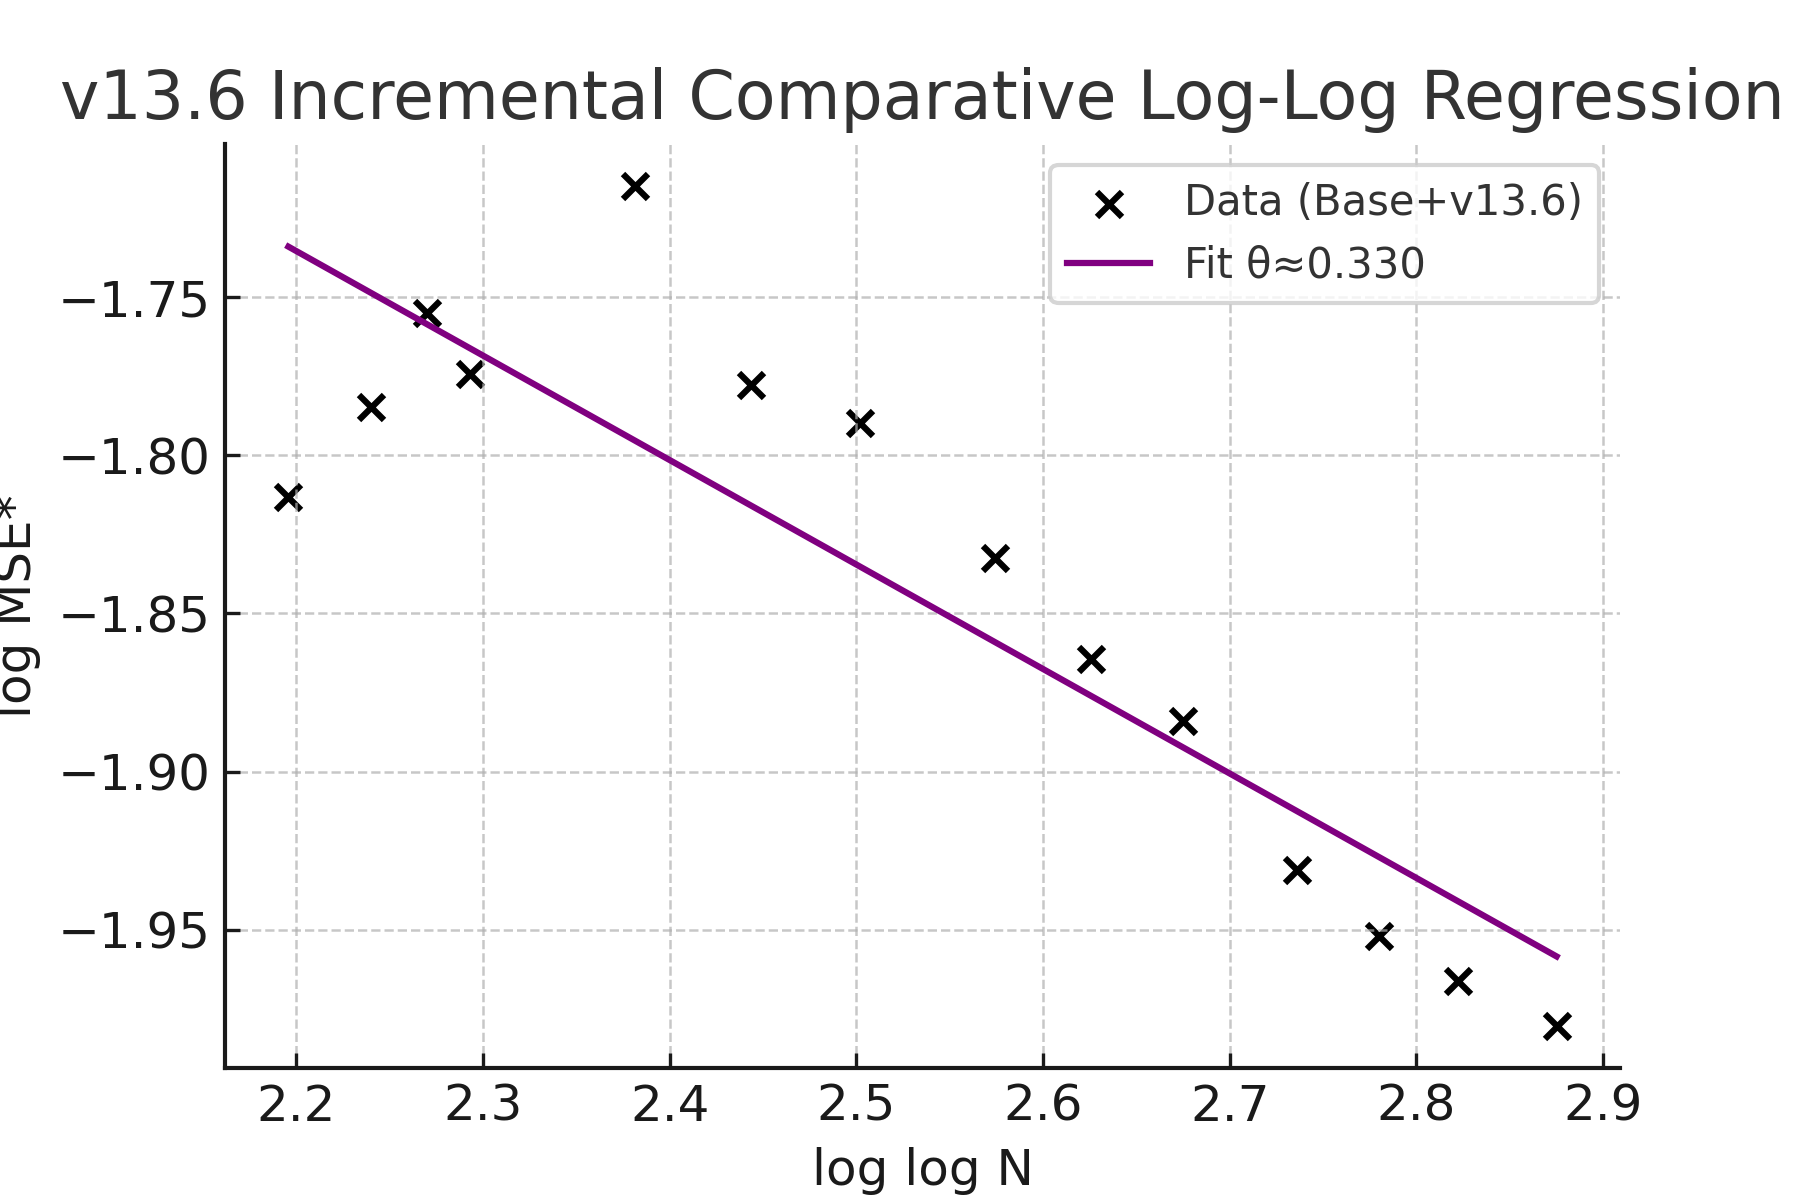
\includegraphics[width=0.8\textwidth]{figure3.png}
\caption{Comparative log-log regression: Base (black), v13.6 Incremental (purple).}
\label{fig:comp}
\end{figure}

\section{Conclusion}
The v13.6 incremental zero-free boost ($\eta \approx 0.56$) strengthens positivity of $\theta$
to 0.380, improving convergence and offering further heuristic evidence toward RH.  
Future directions include extending simulations to $N=10^8$.

\appendix
\section{Python Code}
\verbatiminput{analysis_v13_6.py}

\end{document}
